% Options for packages loaded elsewhere
\PassOptionsToPackage{unicode}{hyperref}
\PassOptionsToPackage{hyphens}{url}
\documentclass[
  catalan,
  a4paper,
]{article}
\usepackage{xcolor}
\usepackage[margin=1in]{geometry}
\usepackage{amsmath,amssymb}
\setcounter{secnumdepth}{-\maxdimen} % remove section numbering
\usepackage{iftex}
\ifPDFTeX
  \usepackage[T1]{fontenc}
  \usepackage[utf8]{inputenc}
  \usepackage{textcomp} % provide euro and other symbols
\else % if luatex or xetex
  \usepackage{unicode-math} % this also loads fontspec
  \defaultfontfeatures{Scale=MatchLowercase}
  \defaultfontfeatures[\rmfamily]{Ligatures=TeX,Scale=1}
\fi
\usepackage{lmodern}
\ifPDFTeX\else
  % xetex/luatex font selection
\fi
% Use upquote if available, for straight quotes in verbatim environments
\IfFileExists{upquote.sty}{\usepackage{upquote}}{}
\IfFileExists{microtype.sty}{% use microtype if available
  \usepackage[]{microtype}
  \UseMicrotypeSet[protrusion]{basicmath} % disable protrusion for tt fonts
}{}
\usepackage{setspace}
\makeatletter
\@ifundefined{KOMAClassName}{% if non-KOMA class
  \IfFileExists{parskip.sty}{%
    \usepackage{parskip}
  }{% else
    \setlength{\parindent}{0pt}
    \setlength{\parskip}{6pt plus 2pt minus 1pt}}
}{% if KOMA class
  \KOMAoptions{parskip=half}}
\makeatother
\usepackage{longtable,booktabs,array}
\usepackage{calc} % for calculating minipage widths
% Correct order of tables after \paragraph or \subparagraph
\usepackage{etoolbox}
\makeatletter
\patchcmd\longtable{\par}{\if@noskipsec\mbox{}\fi\par}{}{}
\makeatother
% Allow footnotes in longtable head/foot
\IfFileExists{footnotehyper.sty}{\usepackage{footnotehyper}}{\usepackage{footnote}}
\makesavenoteenv{longtable}
\usepackage{graphicx}
\makeatletter
\newsavebox\pandoc@box
\newcommand*\pandocbounded[1]{% scales image to fit in text height/width
  \sbox\pandoc@box{#1}%
  \Gscale@div\@tempa{\textheight}{\dimexpr\ht\pandoc@box+\dp\pandoc@box\relax}%
  \Gscale@div\@tempb{\linewidth}{\wd\pandoc@box}%
  \ifdim\@tempb\p@<\@tempa\p@\let\@tempa\@tempb\fi% select the smaller of both
  \ifdim\@tempa\p@<\p@\scalebox{\@tempa}{\usebox\pandoc@box}%
  \else\usebox{\pandoc@box}%
  \fi%
}
% Set default figure placement to htbp
\def\fps@figure{htbp}
\makeatother
\ifLuaTeX
\usepackage[bidi=basic]{babel}
\else
\usepackage[bidi=default]{babel}
\fi
% get rid of language-specific shorthands (see #6817):
\let\LanguageShortHands\languageshorthands
\def\languageshorthands#1{}
\setlength{\emergencystretch}{3em} % prevent overfull lines
\providecommand{\tightlist}{%
  \setlength{\itemsep}{0pt}\setlength{\parskip}{0pt}}
\usepackage{bookmark}
\IfFileExists{xurl.sty}{\usepackage{xurl}}{} % add URL line breaks if available
\urlstyle{same}
\hypersetup{
  pdftitle={U5. DEBIAN. INSTAL·LACIÓ MÍNIMA},
  pdfauthor={@tofermos 2026},
  pdflang={ca-ES},
  hidelinks,
  pdfcreator={LaTeX via pandoc}}

\title{U5. DEBIAN. INSTAL·LACIÓ MÍNIMA}
\author{@tofermos 2026}
\date{}

\begin{document}
\maketitle

{
\setcounter{tocdepth}{2}
\tableofcontents
}
\setstretch{1.5}
\newpage
\renewcommand\tablename{Tabla}

\section{1. Instal·lar Debian sense entorn
gràfic}\label{installar-debian-sense-entorn-gruxe0fic}

Triem l'opció d'instal·lador gràfic (no instal·larem el GUI)

\begin{figure}
\centering
\pandocbounded{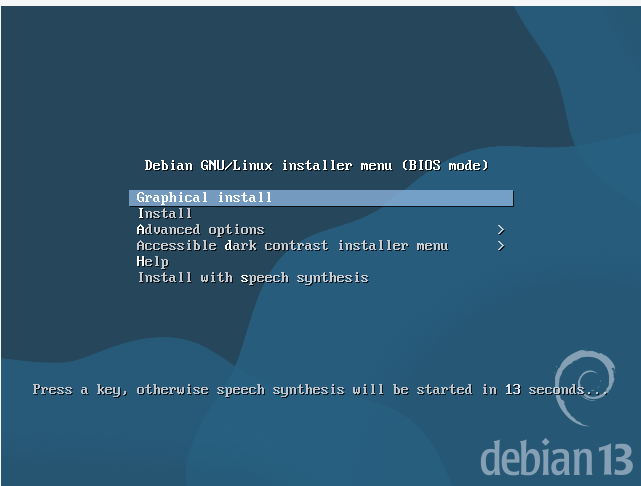
\includegraphics[keepaspectratio]{png/debian/Debian1.png}}
\caption{\emph{Figura 1: Instal·lació gràfica}}
\end{figure}

\begin{figure}
\centering
\pandocbounded{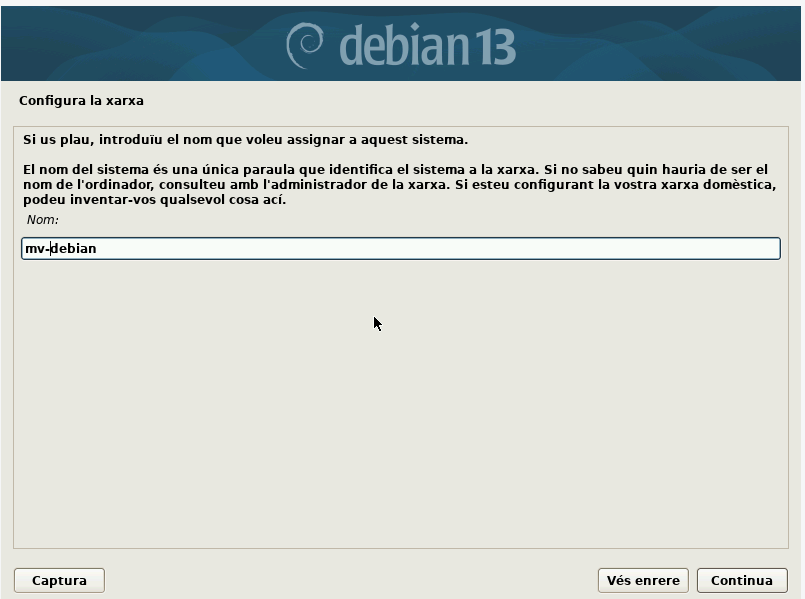
\includegraphics[keepaspectratio]{png/debian/Debian03nommaquina.png}}
\caption{\emph{Figura 2: Nom del PC}}
\end{figure}

Les instal·lacions d'Ubuntu deixen, per defecte, l'usuari root
inhabilitat i no apareix esta opció. La de Debian, ens dóna l'opció
d'habilitar-lo. No obstant, de moment no ho farem i, per a aixó,
deixarem en blanc els camps de contrassenya.

\begin{figure}
\centering
\pandocbounded{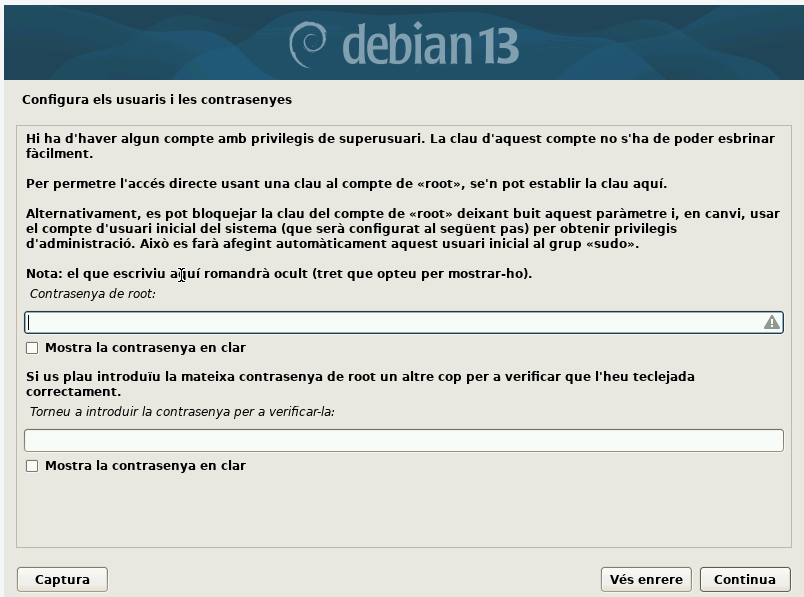
\includegraphics[keepaspectratio]{png/debian/Debian04rootenblanc.png}}
\caption{\emph{Figura 2: root en blanc}}
\end{figure}

\begin{figure}
\centering
\pandocbounded{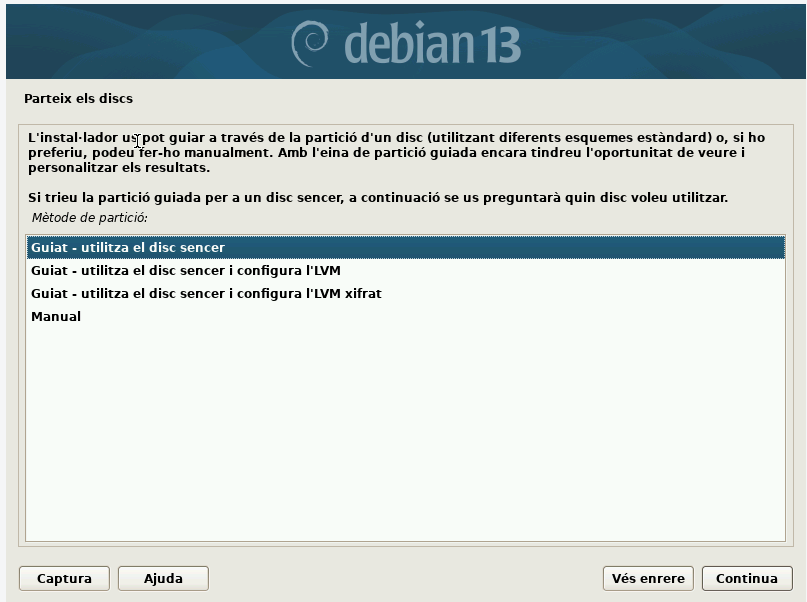
\includegraphics[keepaspectratio]{png/debian/Debian05utilitzadiscsencer.png}}
\caption{\emph{Figura 3: elegim un disc físic}}
\end{figure}

Compte! Trieu correctament el disc on instal·lar. Apareixeran tots els
dispositius de magatzenament secundari: discos durs interns, externs,
pendrives\ldots{} (sdX, nvmeX, hdX\ldots)

\begin{figure}
\centering
\pandocbounded{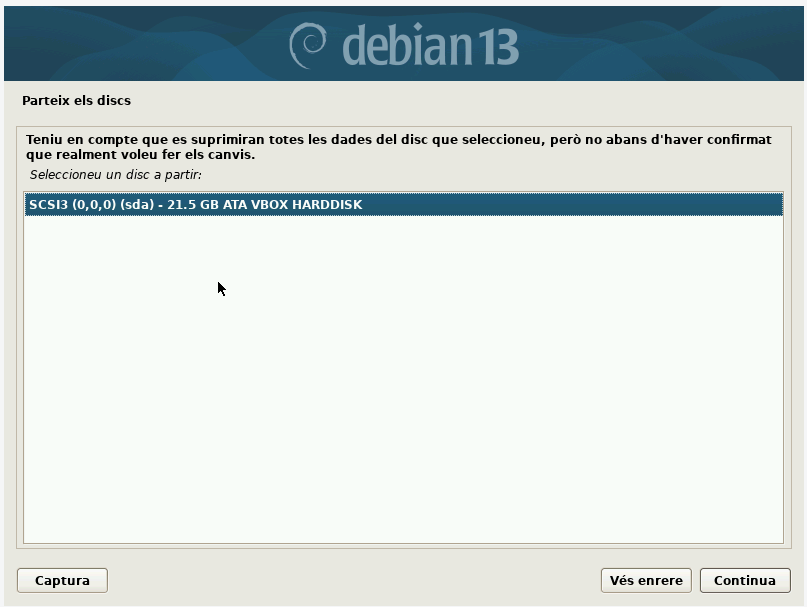
\includegraphics[keepaspectratio]{png/debian/Debian06seleccionadisc.png}}
\caption{\emph{Figura 3: Seleccionem el disc on instal·larem}}
\end{figure}

\begin{figure}
\centering
\pandocbounded{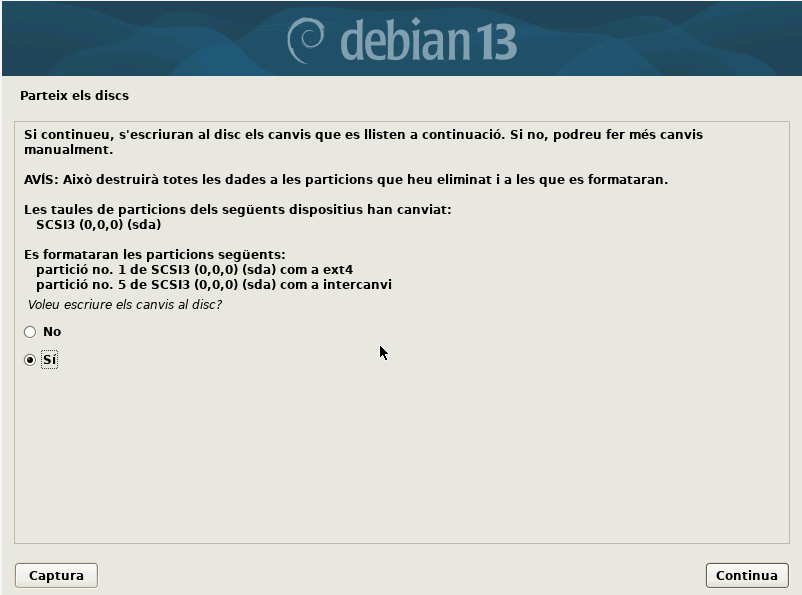
\includegraphics[keepaspectratio]{png/debian/Debian07confirmadisc.png}}
\caption{\emph{Figura 4: Seleccionem el disc on instal·larem}}
\end{figure}

\begin{figure}
\centering
\pandocbounded{\includegraphics[keepaspectratio]{png/debian/Debian07paricions.png}}
\caption{\emph{Figura 5: Seleccionem particions}}
\end{figure}

\begin{figure}
\centering
\pandocbounded{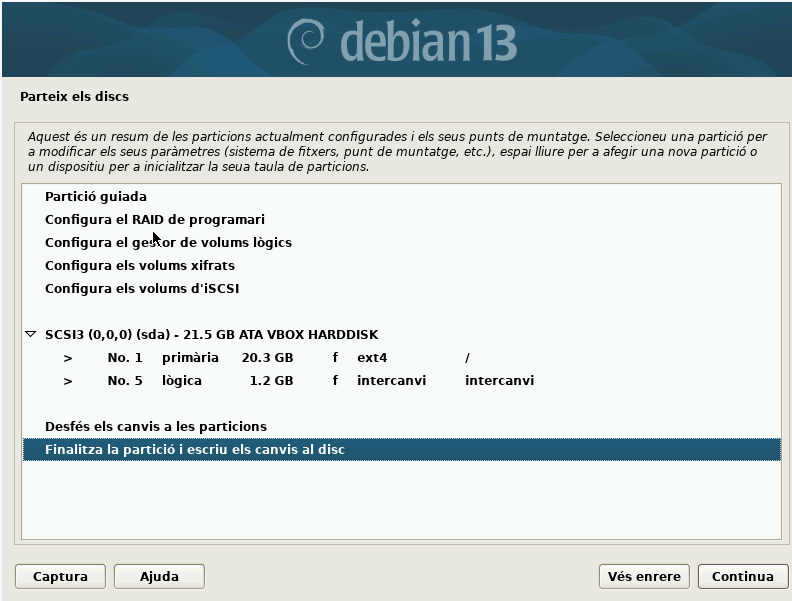
\includegraphics[keepaspectratio]{png/debian/Debian10confirmacanvis.png}}
\caption{\emph{Figura 6: Confirma}}
\end{figure}

\begin{figure}
\centering
\pandocbounded{\includegraphics[keepaspectratio]{png/debian/Debian12replica.png}}
\caption{\emph{Figura 7: Replica}}
\end{figure}

\begin{figure}
\centering
\pandocbounded{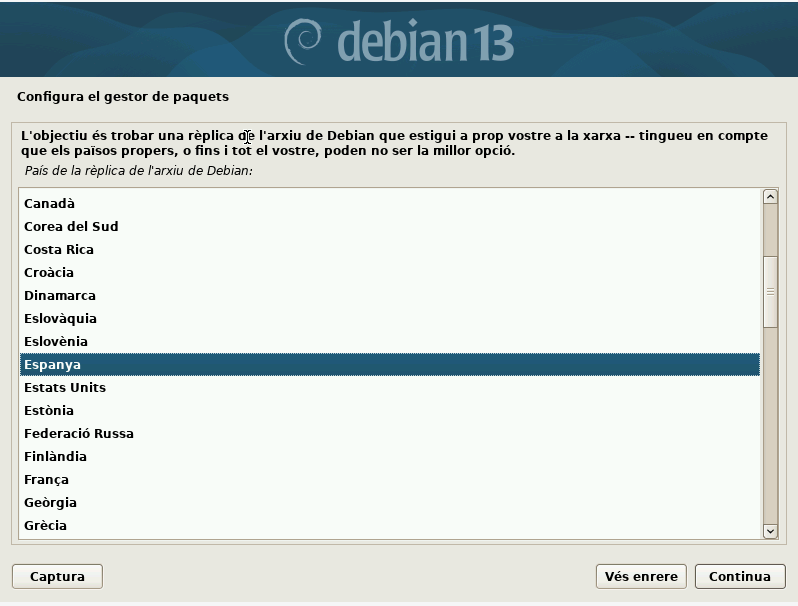
\includegraphics[keepaspectratio]{png/debian/Debian12replica1.png}}
\caption{\emph{Figura 8: Replica}}
\end{figure}

\begin{figure}
\centering
\pandocbounded{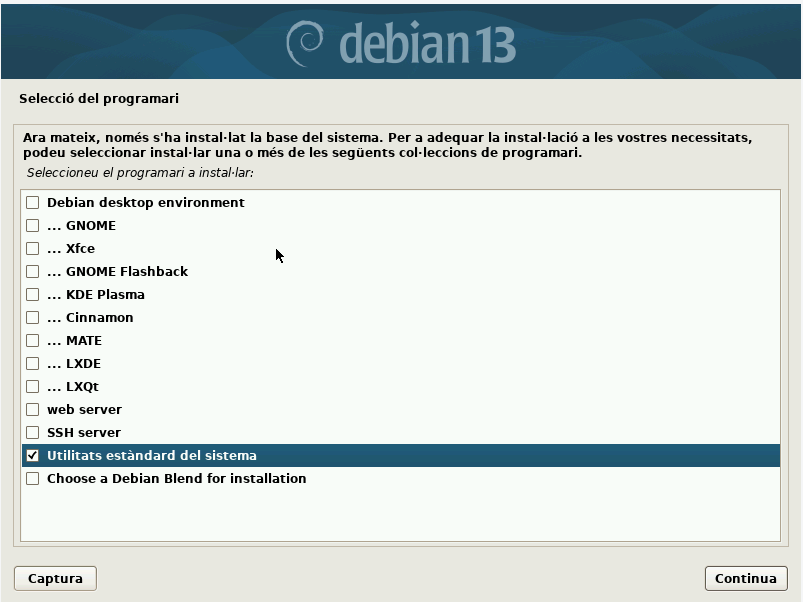
\includegraphics[keepaspectratio]{png/debian/Debian13escriptori.png}}
\caption{\emph{Figura 9: Replica}}
\end{figure}

\begin{figure}
\centering
\pandocbounded{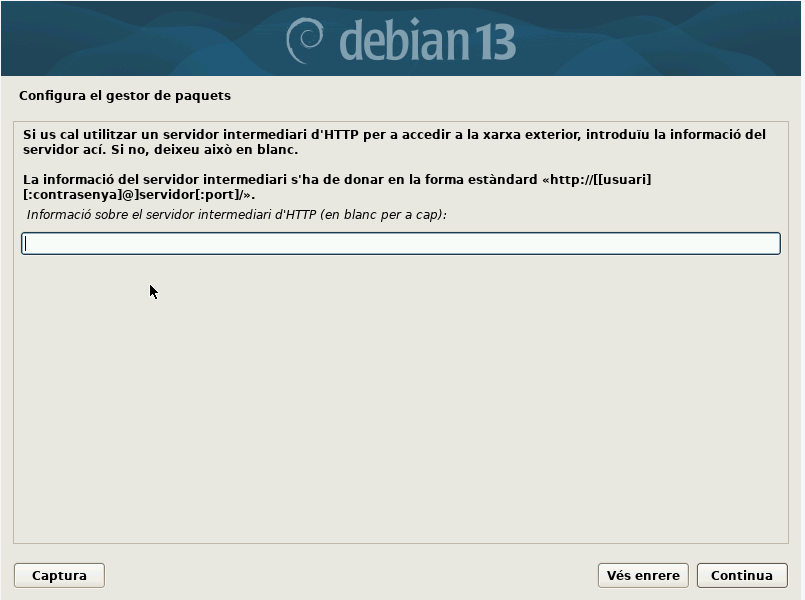
\includegraphics[keepaspectratio]{png/debian/Debian13http.png}}
\caption{\emph{Figura 10: Sense http}}
\end{figure}

\begin{figure}
\centering
\pandocbounded{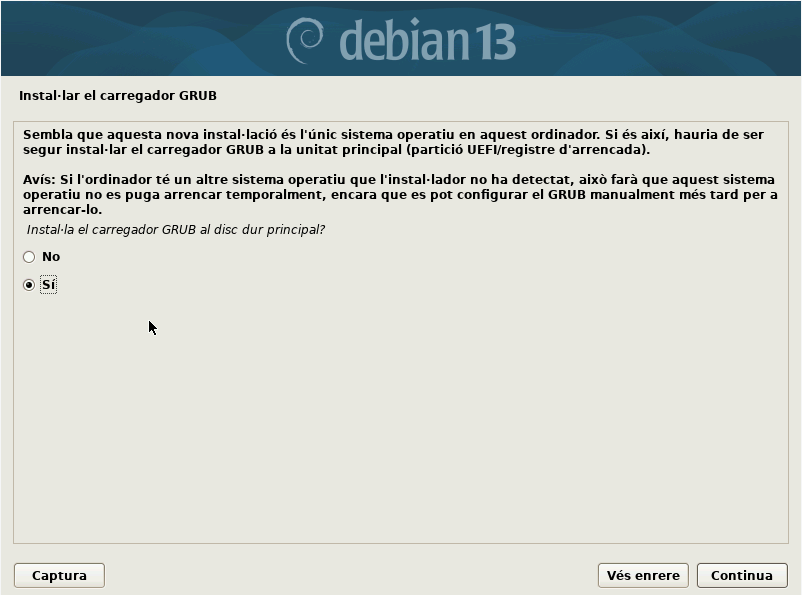
\includegraphics[keepaspectratio]{png/debian/Debian14grub.png}}
\caption{\emph{Figura 11: Replica}}
\end{figure}

\begin{figure}
\centering
\pandocbounded{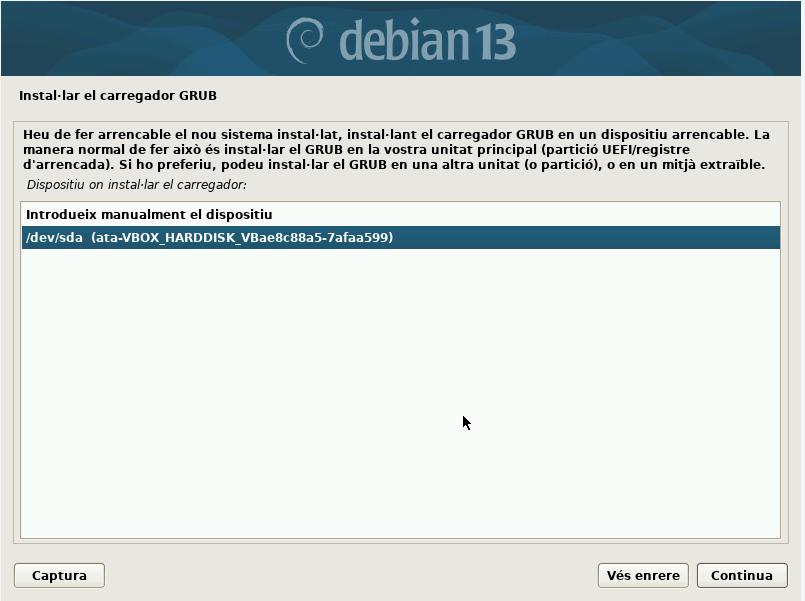
\includegraphics[keepaspectratio]{png/debian/Debian15grub2.png}}
\caption{\emph{Figura 12: Replica}}
\end{figure}

\section{2. Afegir GUI Mínim}\label{afegir-gui-muxednim}

\begin{longtable}[]{@{}
  >{\raggedright\arraybackslash}p{(\linewidth - 2\tabcolsep) * \real{0.3333}}
  >{\raggedright\arraybackslash}p{(\linewidth - 2\tabcolsep) * \real{0.6667}}@{}}
\toprule\noalign{}
\begin{minipage}[b]{\linewidth}\raggedright
Paquet
\end{minipage} & \begin{minipage}[b]{\linewidth}\raggedright
Descripció
\end{minipage} \\
\midrule\noalign{}
\endhead
\bottomrule\noalign{}
\endlastfoot
Xorg & Procés del servidor gràfic X11; permet la comunicació amb
pantalla i dispositius d'entrada \\
Openbox & Gestor de finestres: disposició, vores, moviment, menús i
escriptoris. \\
startx / xinit & Mecanisme que arranca Xorg i la sessió indicada a
\textasciitilde/.xinitrc; no és un escriptori. \\
Firefox / xterm & Aplicacions gràfiques: són clients X11; Openbox
administra les seues finestres. \\
LightDM (no instal·lat) & Alternativa gràfica per autenticar-se i
iniciar sessions, innecessària per a aquesta pràctica. \\
\end{longtable}

Instal·lem els tres paquets al mateix temps.

\begin{verbatim}
sudo apt update
sudo apt install --no-install-recommends xorg openbox xinit xterm
\end{verbatim}

Preparem com iniciar el GUI des del CLI.

Creant un fitxer

\begin{verbatim}
nano ~/.xinitrc
\end{verbatim}

\begin{enumerate}
\def\labelenumi{\arabic{enumi}.}
\tightlist
\item
  Escriure \textbf{openbox-session}
\item
  Guardar amb Control X
\end{enumerate}

Ja podem inicar el CLI amb

\begin{verbatim}
startx
\end{verbatim}

\section{3 Instal·lar un navegador}\label{installar-un-navegador}

Instal·lem el Firefox

\begin{verbatim}
sudo apt install firefox-esr
\end{verbatim}

\end{document}
